\section{Binární halda}\label{sec:halda}
Uveďme motivační příklad na úvod. Mějme seznam čísel, z něhož chceme (pokud možno co nejrychleji) vybrat minimální/maximální hodnotu. Pro maximum bychom sestavit následující jednoduchý algoritmus.
\begin{pseudo}{Max}[Seznam čísel $x_1,x_2,\dots,x_n$][Maximální hodnota seznamu \textit{m}]
    $m\gets x_1$\\
    \begin{For}{$i=1,2,\dots,n$}
        \begin{If}{$x_i>m$}
            $m\gets x_i$
        \end{If}
    \end{For}
\end{pseudo}

Časová složitost bude zjevně $\bigO{n}$, neboť algoritmus prochází všech $n$ prvků. Takovou úlohu lze však řešit rychleji, pokud si prvky vhodně uspořádáme. K tomu můžeme použít tzv. \emph{haldu}. 
\begin{definition}[Minimová binární halda]\label{def:binarni_halda}
    Minimová binární halda je datová struktura tvaru binárního stromu, kde v každém vrcholu je uložena \emph{právě jedna} hodnota (tzv. \emph{klíč}, pro vrchol $v$ budeme značit jeho klíč $k(v)$) a navíc platí:
    \begin{enumerate}[label=(\roman*)]
        \item\label{binhalda_podminka_1} každá hladina je \emph{plně obsazena}, kromě poslední, pričemž hladiny jsou zaplněny \emph{zleva}
        \item\label{binhalda_podminka_2} a je-li $v$ libovolný vrchol a $s$ jeho syn, pak $k(v)\leqslant k(s)$.
    \end{enumerate}
\end{definition}

\begin{figure}[h]
    \centering
    \begin{subfigure}{6cm}
        \centering
        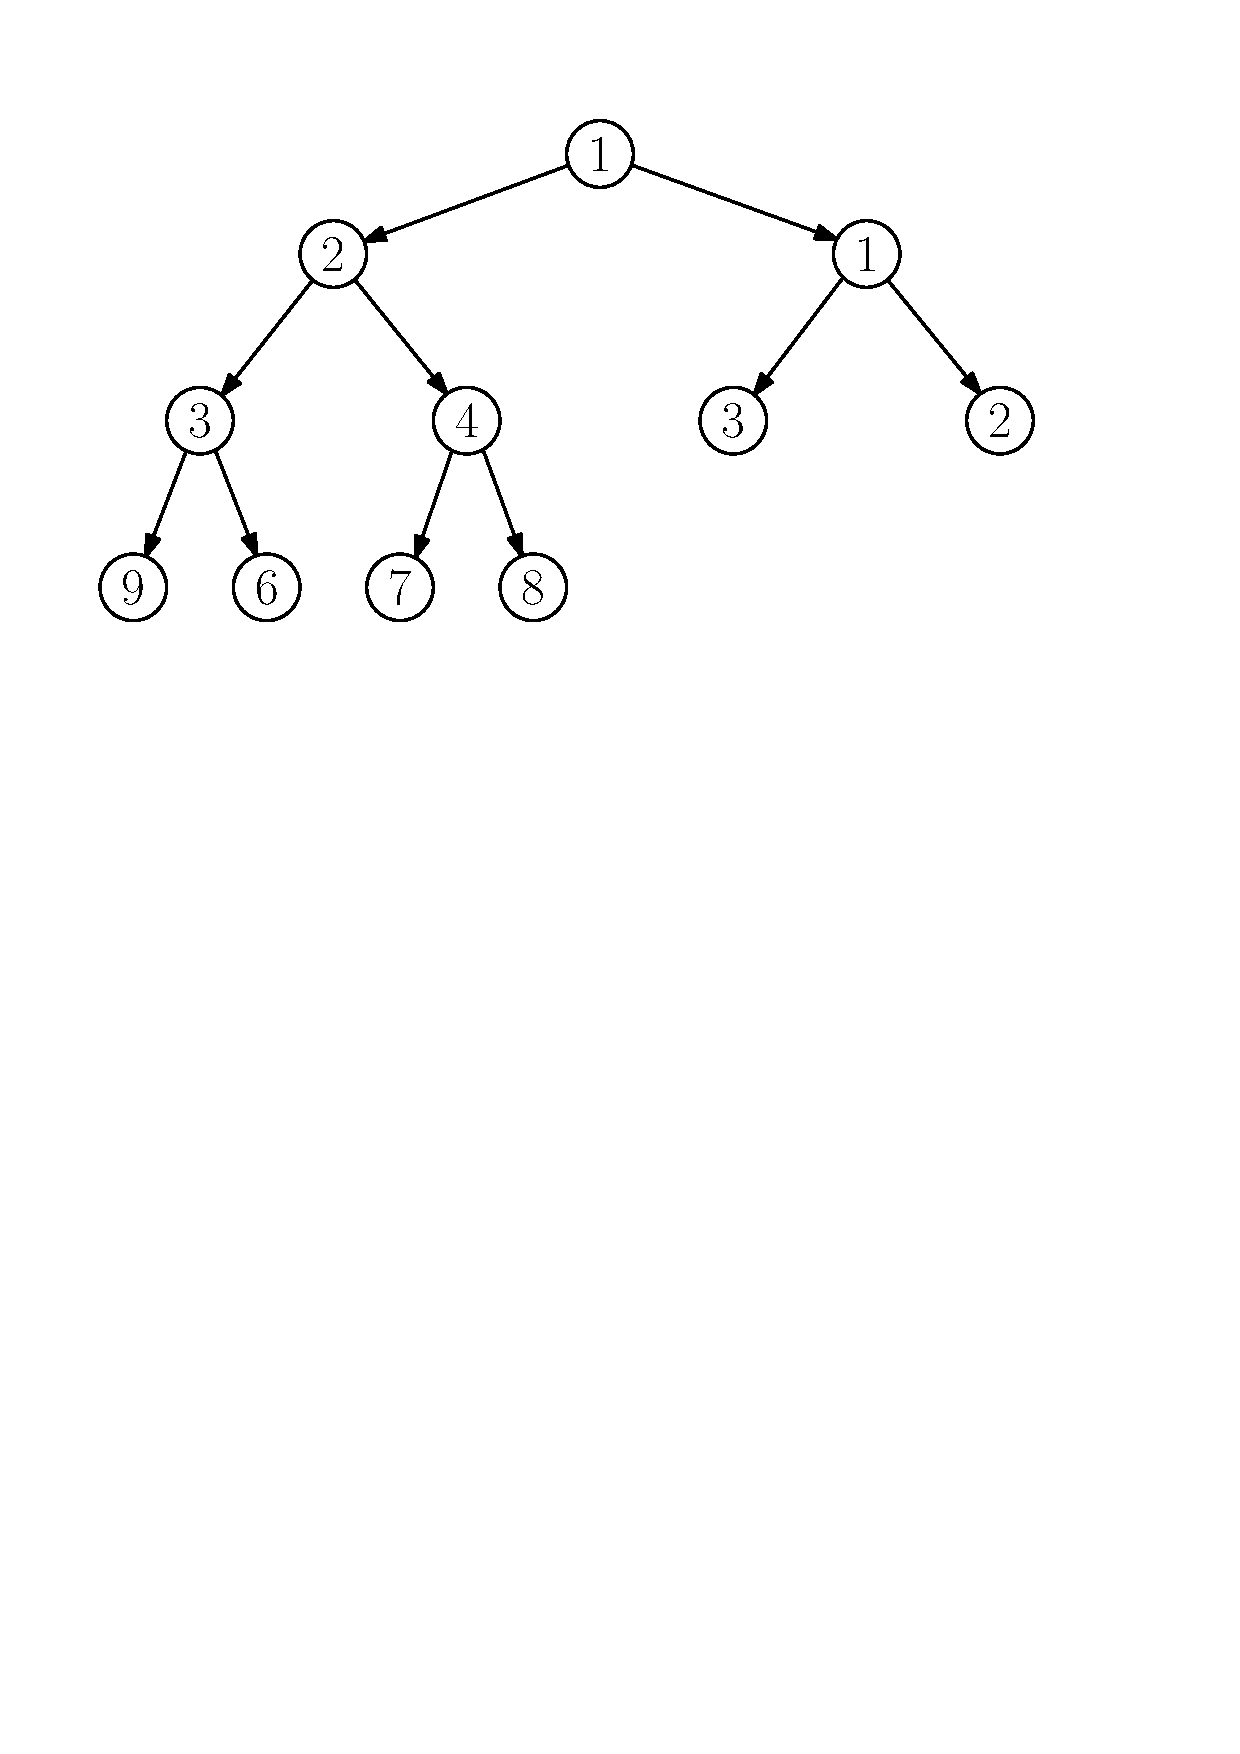
\includegraphics[scale=.4]{ch01_halda}
        \caption{Korektní halda.}
        \label{subfig:korektni_halda}
    \end{subfigure}
    \quad
    \begin{subfigure}{5cm}
        \centering
        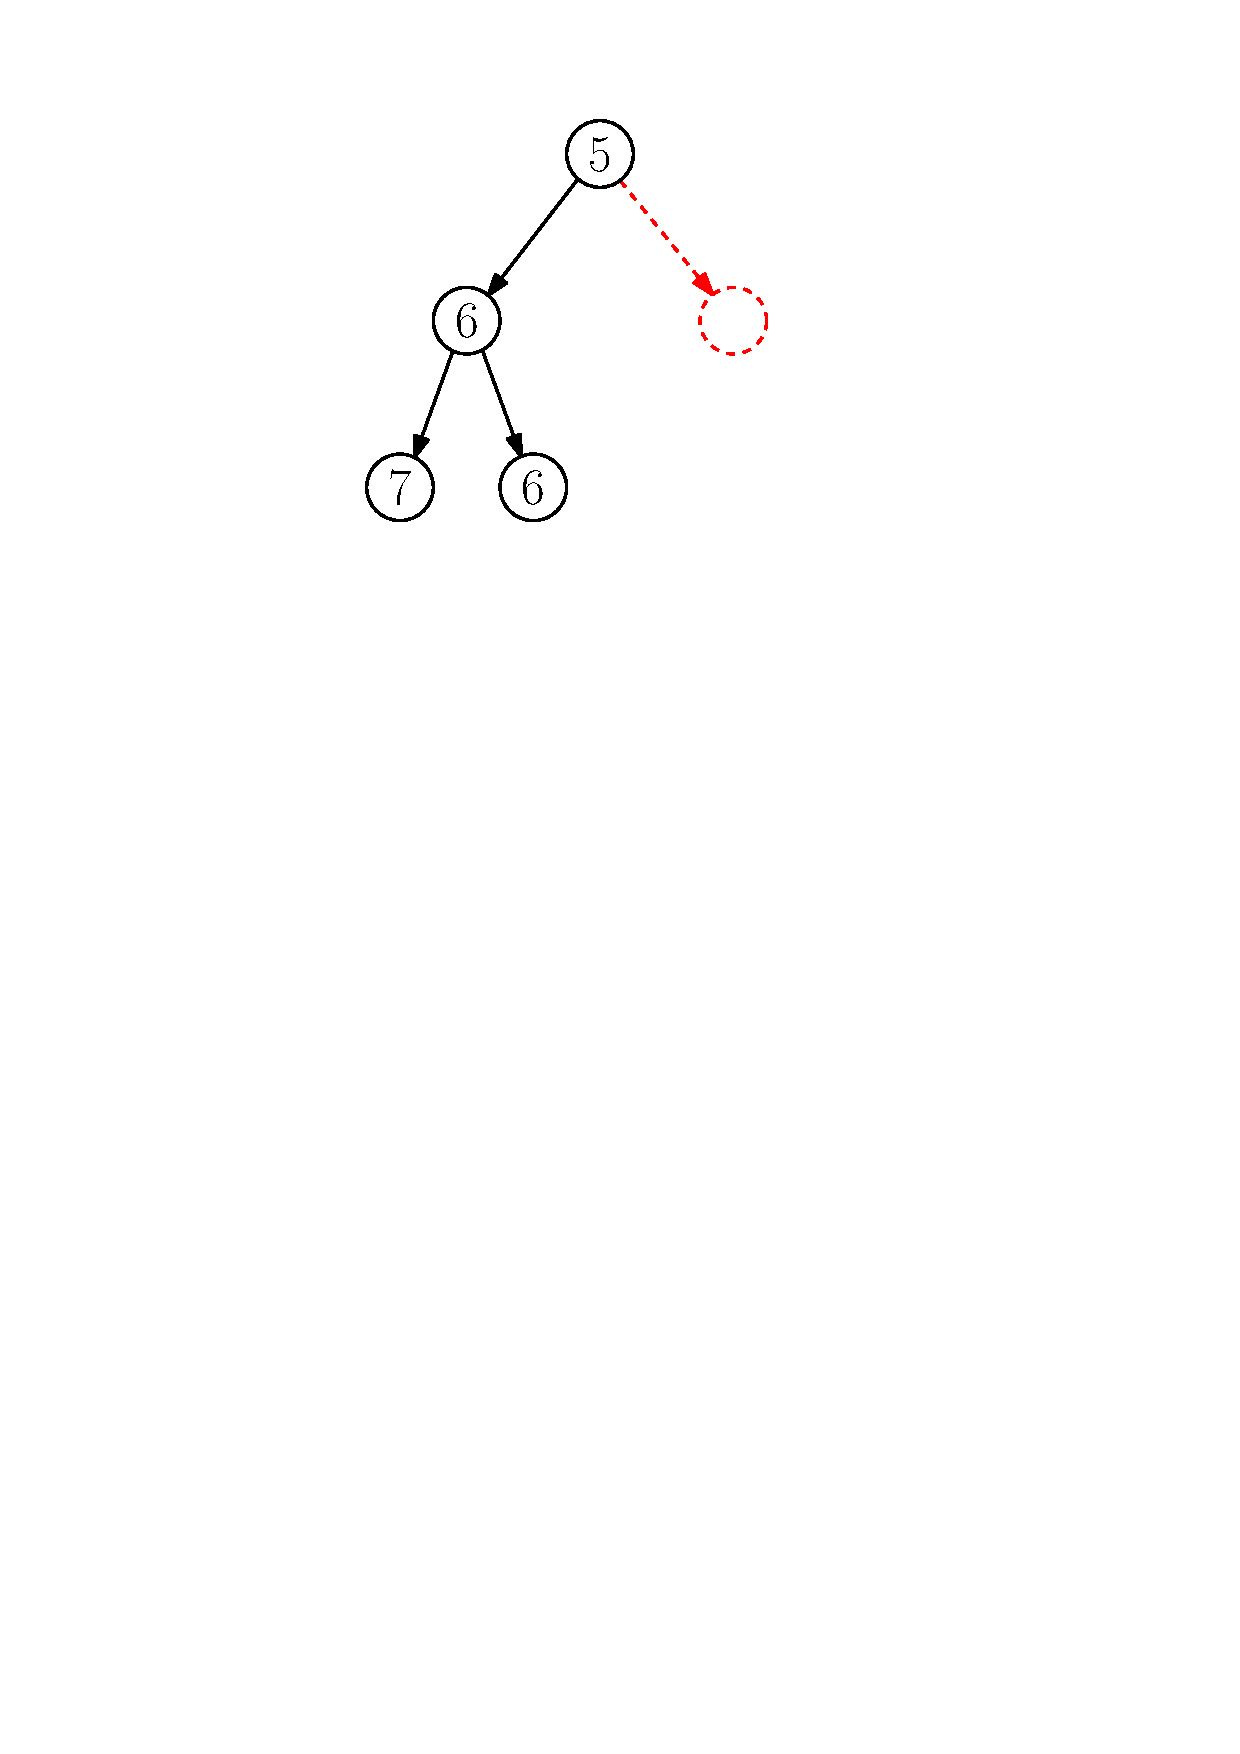
\includegraphics[scale=.4]{ch01_nekor_halda_1}
        \caption{Chybějící vrchol v 1. hladině.}
        \label{subfig:nekorektni_halda_1}
    \end{subfigure}
    \quad
    \begin{subfigure}{5cm}
        \centering
        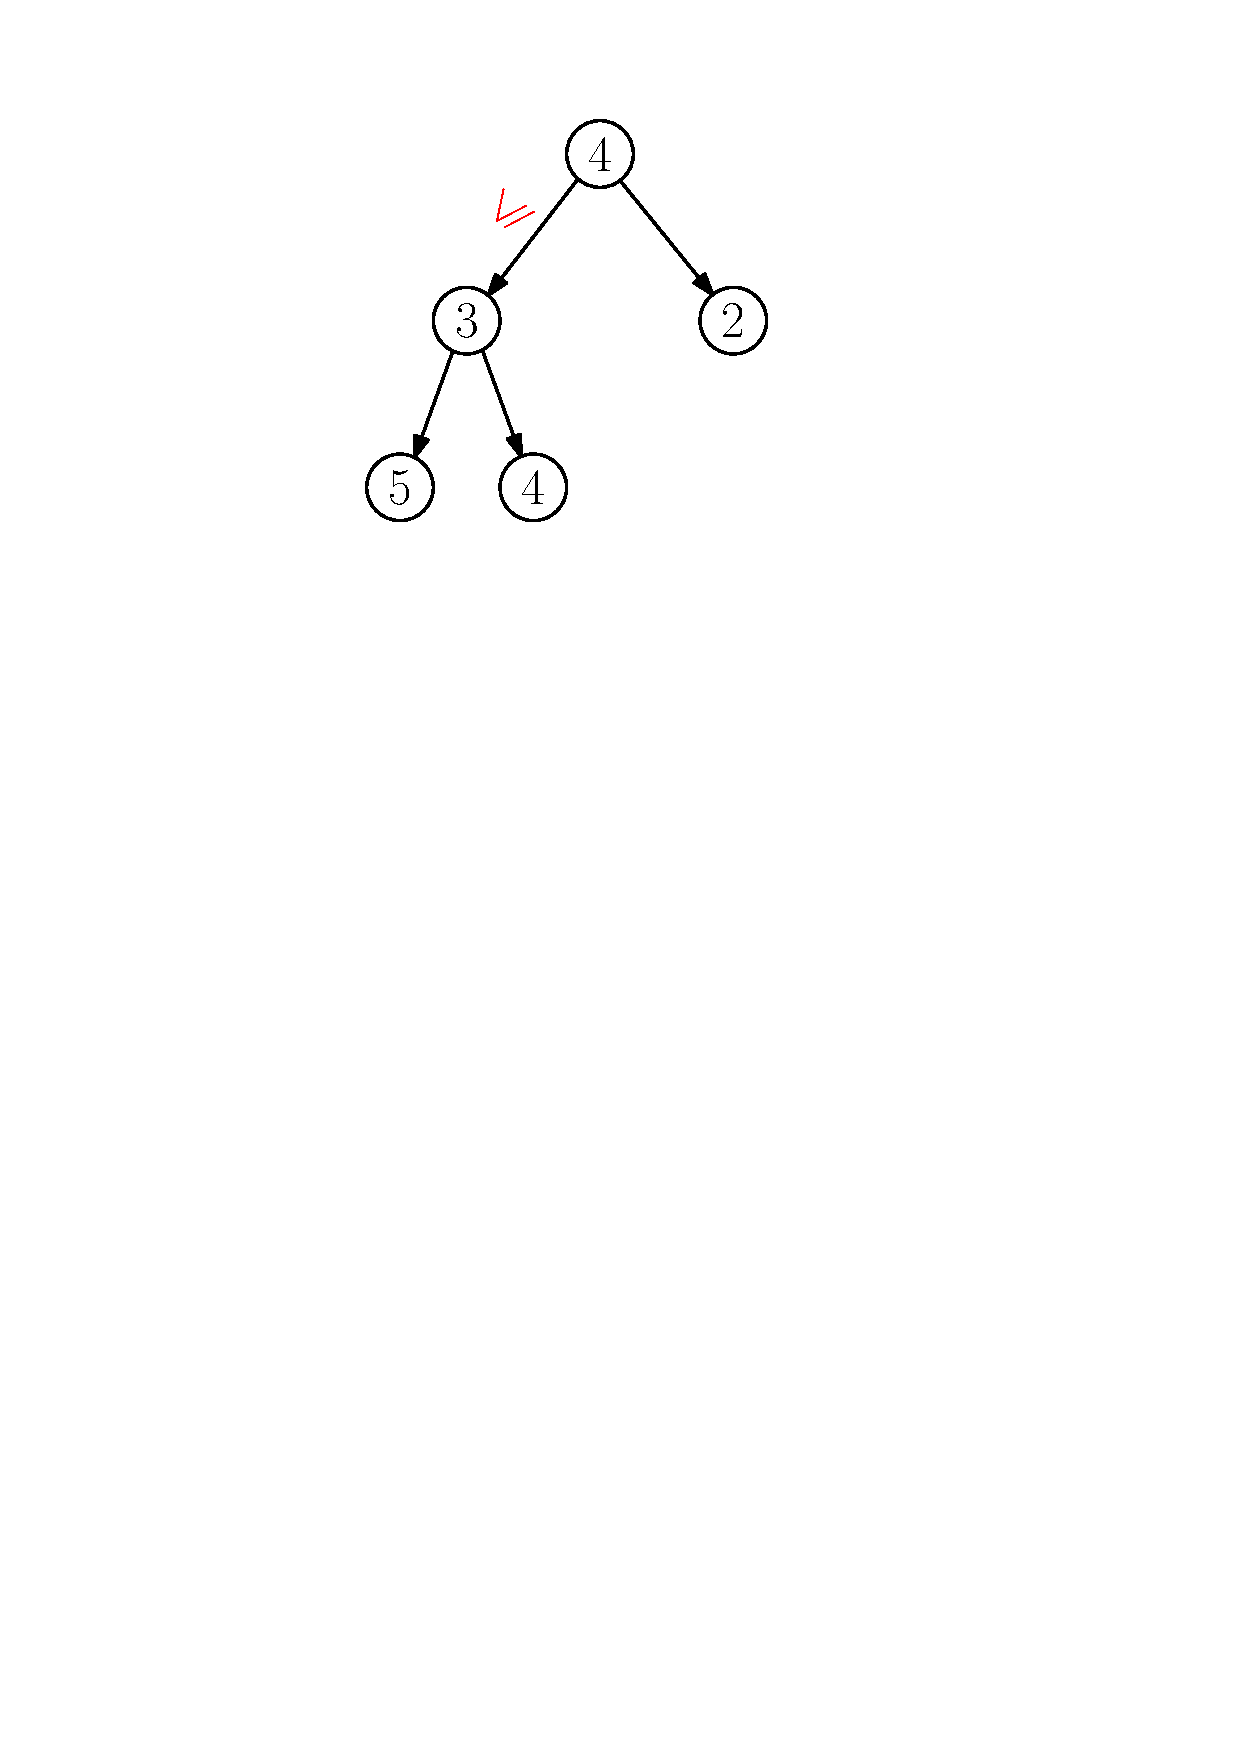
\includegraphics[scale=.4]{ch01_nekor_halda_2}
        \caption{Klíč levého syna je menší než klíč kořene.}
        \label{subfig:nekorektni_halda_2}
    \end{subfigure}
    \caption{Příklady korektních a nekorektních hald.}
    \label{fig:halda_modely}
\end{figure}

Zde se nyní na chvíli pozastavme. Podmínka \ref{binhalda_podminka_2} v definici binární haldy \ref{def:binarni_halda} má za následek totiž velmi příjemnou vlastnost, když se podíváme, kde se v haldě nachází minimum. Pokud se budeme pohybovat od kořene směrem "dolů", hodnoty ve vrcholech se budou pouze zvětšovat, neboť klíče synů musí mít vždy stejnou nebo větší hodnotu než klíč v rodiči. Minimum se tak vždy nachází \emph{v kořeni stromu}, což znamená, že zjistění minima tak můžeme provést v \emph{konstantním čase} $\bigO{1}$.
\notebox{Pokud bychom chtěli naopak \emph{maximovou binární haldu}, bude definice \ref{def:binarni_halda} vypadat obdobně, akorát v podmínce \ref{binhalda_podminka_2} bude obrácená nerovnost, tj. $k(v)\geqslant k(s)$ (klíč v rodiči má vždy stejnou nebo vyšší hodnotu než klíče v jeho synech). Maximum se bude opět nacházet v kořeni haldy.}
Je však více operací, které bychom rádi s haldou prováděli. Vypišme si všechny, které nás budou zajímat.
\begin{itemize}
    \item \textsc{Insert}($x$) -- \emph{vložení} nového vrcholu s klíčem $x$ do haldy.
    \item \textsc{Min}() -- \emph{nalezení} vrcholu s nejmenším klíčem (už jsme zmínili).
    \item \textsc{ExtractMin}() -- \emph{odebrání} vrcholu s nejmenším klíčem.
    \item \textsc{Increase}($v$) -- \emph{zvýšení} hodnoty klíče ve zvoleném vrcholu $v$.
    \item \textsc{Decrease}($v$) -- \emph{snížení} hodnoty klíče ve zvoleném vrcholu $v$.
\end{itemize}

Podívejme se postupně na jednotlivé operace a jejich realizaci. S dovolením si zde nyní odpustíme zápis pomocí pseudokódu a pro jednoduchost si dané operace pouze slovně vysvětlíme. Pro následné odvození časové složitosti nám to bude stačit.

\subsubsection{Vkládání nového vrcholu}

Při vkládání nového vrcholu (\textsc{Insert}) se nejdříve potřebujeme vypořádat s tím, kam vrchol v haldě umístíme. S tím nám ale pomůže podmínka \ref{binhalda_podminka_1} v definici binární haldy. Všechny hladiny stromu jsou vždy plně obsazené, kromě poslední, která se všechny vrcholy nachází vlevo. To znamená, že nový vrchol můžeme umístit na první volnou pozici vlevo na poslední hladině. To však nemůžeme provést zcela beztrestně, neboť nemáme nijak zaručeno, že bude splněna podmínka \ref{binhalda_podminka_2}. Klíč v novém vrcholu může mít hodnotu \emph{ostře menší} než jeho rodič. Haldu "opravíme" postupným prohazováním vrcholu s jeho rodičem, dokud nebude podmínka splněna (viz obrázek \ref{fig:vkladani_vrcholu_halda}).
\begin{figure}[h]
    \centering
    \begin{subfigure}{7cm}
        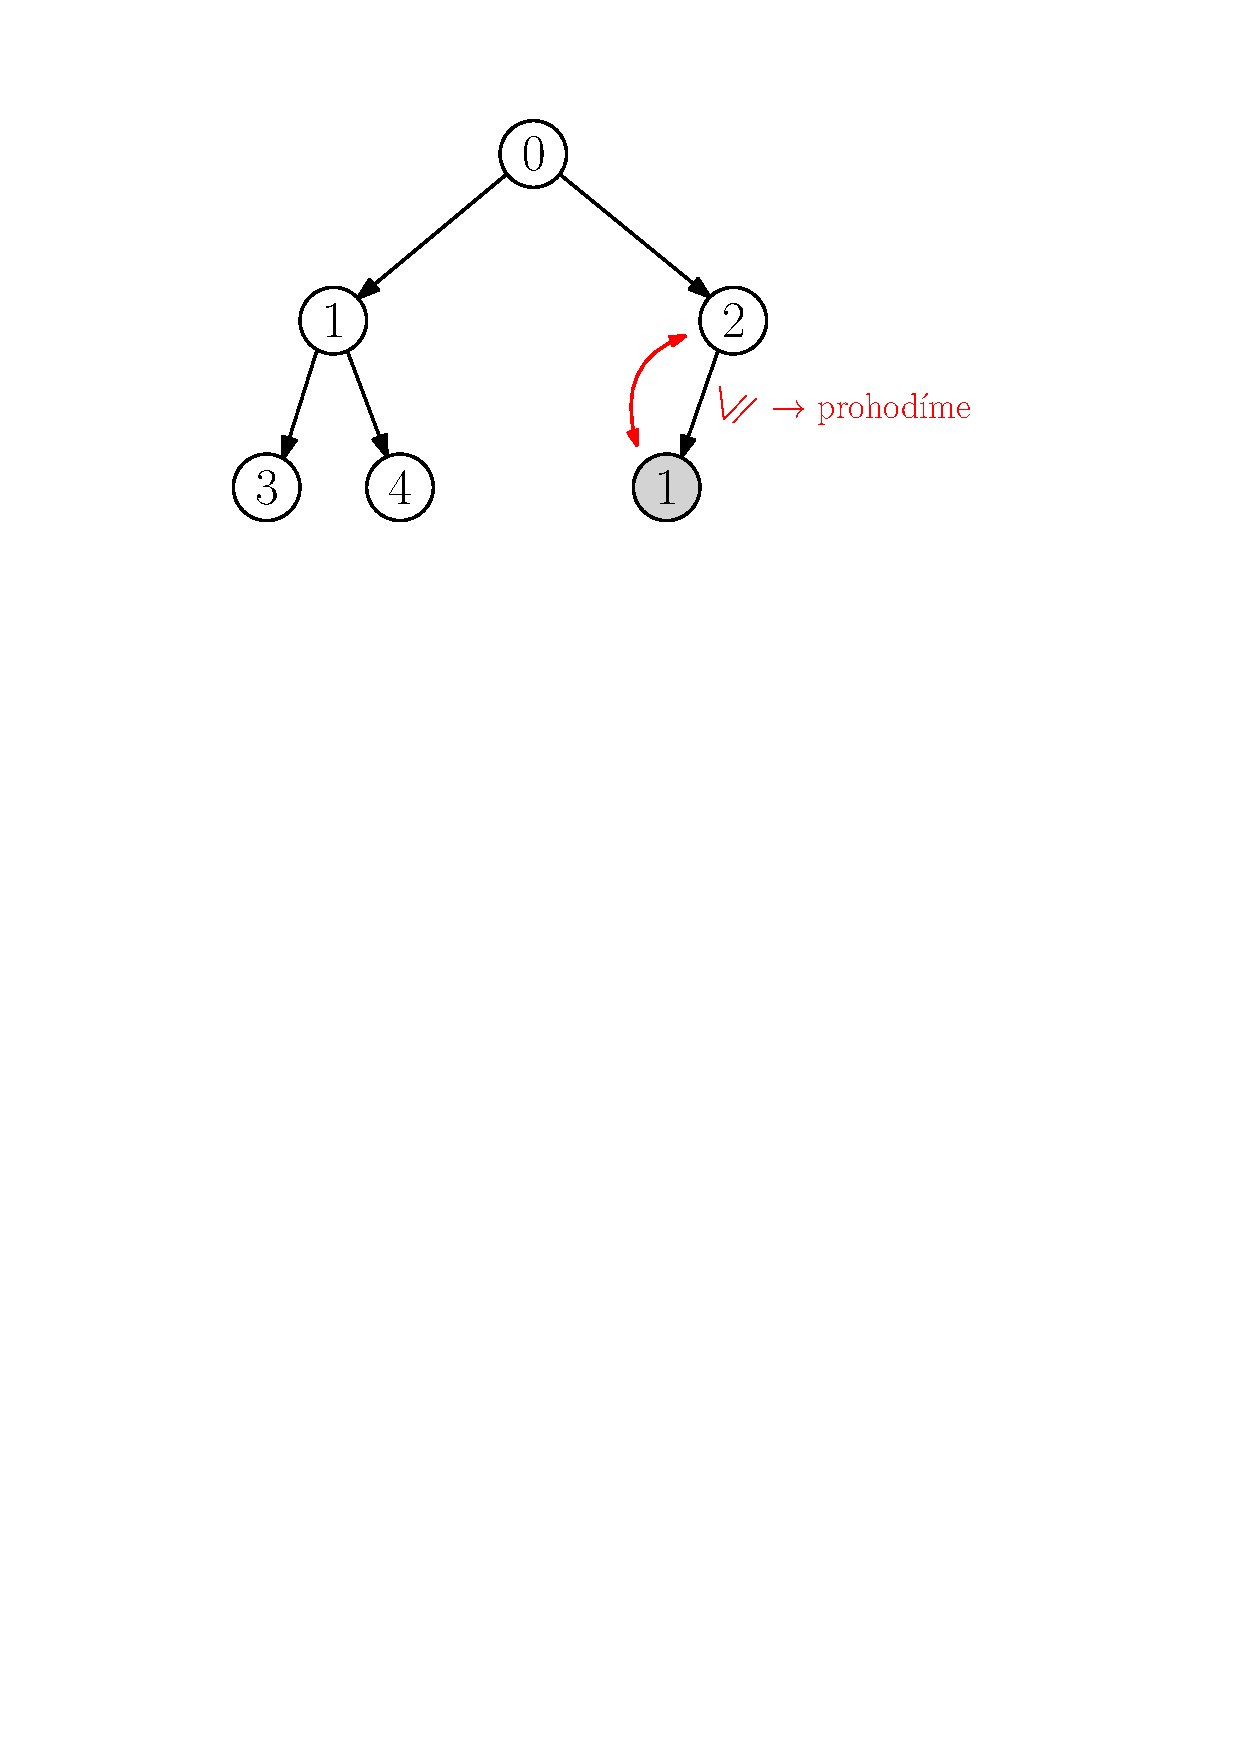
\includegraphics[scale=.5]{ch01_vkladani_1}
    \end{subfigure}
    \begin{subfigure}{7cm}
        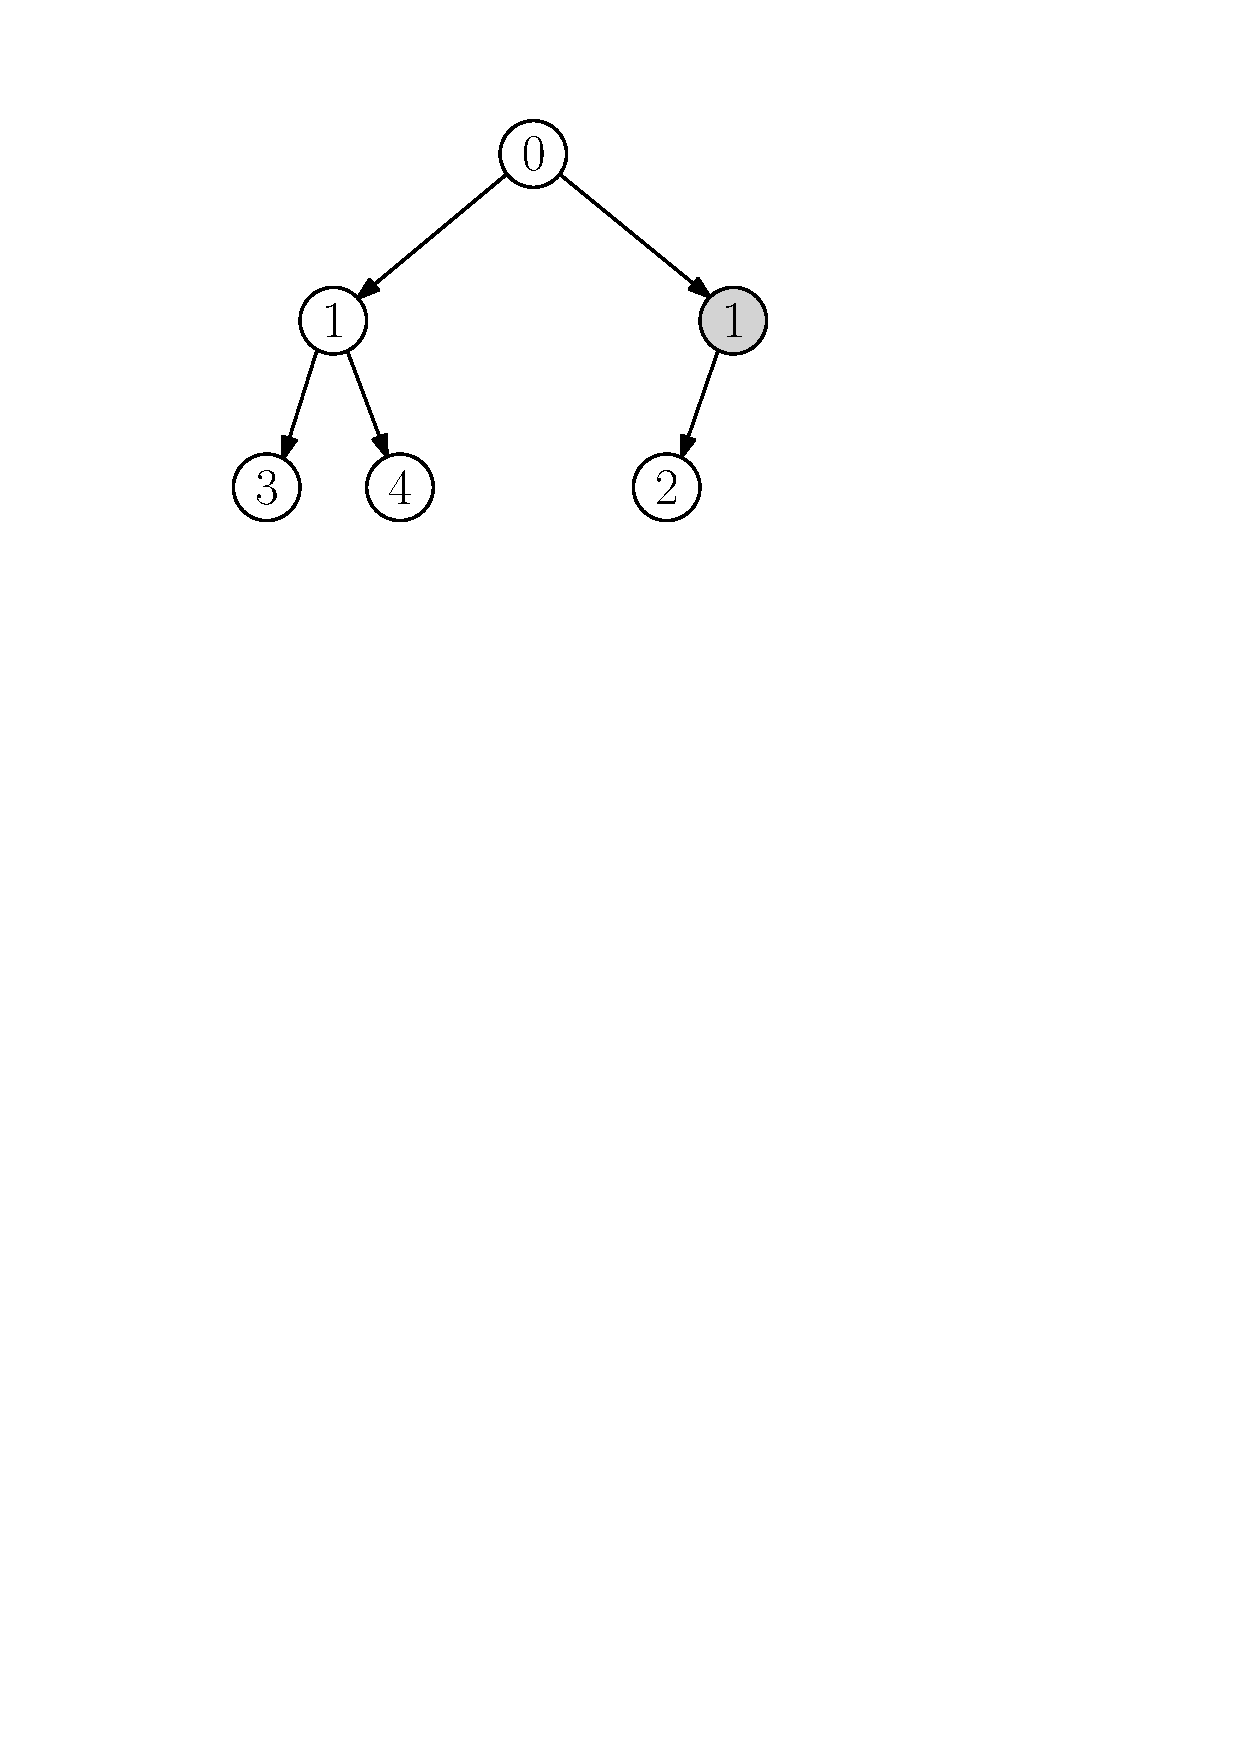
\includegraphics[scale=.5]{ch01_vkladani_2}
    \end{subfigure}
    \caption{Vkládání nového vrcholu do haldy.}
    \label{fig:vkladani_vrcholu_halda}
\end{figure}
Postup můžeme zapsat zkráceně ve třech bodech takto:
\begin{itemize}
    \item Vložíme nový vrchol s klíčem $x$ na první volnou pozici zleva na poslední hladině.
    \item pokud je klíč rodiče větší než $x$, prohodíme vrcholy (resp. jejich klíče)\footnote{Vrchol v podstatě takto "probublá" do správné pozice ve stromě (příp. až do pozice kořene).}.
    \item Opakujeme druhý krok.
\end{itemize}

\subsubsection{Odstranění minima}

Co se týče získání minimálního klíče v haldě, jedná se o velmi triviální operaci. Zkrátka "přečteme" klíč v kořeni a jsme hotovi. Ovšem pokud bychom chtěli minimum (\textsc{ExtractMin}) ze stromu odstanit, bude to již o něco složtější. Kořen ze stromu nemůžeme "jen tak" smazat, jeho pozici musí zastoupit jiný vrchol. Abychom neporušili vlastnosti haldy, nahradíme odstraněný kořen \emph{nejlevějším vrcholem na poslední hladině}. Tím jsme jistě neporušili vlastnost \ref{binhalda_podminka_1}, neboť poslední hladina, jako jediná, nemusí být plně obsazená.

Nyní však (stejně jako u vkládání vrcholu) nastavá problém s druhou podmínkou, neboť touto operací jsme ji mohli porušit. Provedeme obdobný proces, jako pri vkládání vrcholu do haldy, ale vrchol nyní bude "probublávat" směrem dolů. Podíváme se na syny daného vrcholu a pokud klíč některého z nich je menší než klíč nového kořene, pak jej s ním prohodíme (v případě, že klíče obou synů jsou menší, než klíč kořene, prohodíme s menším z nich).
\begin{figure}[h]
    \centering
    \begin{subfigure}{5cm}
        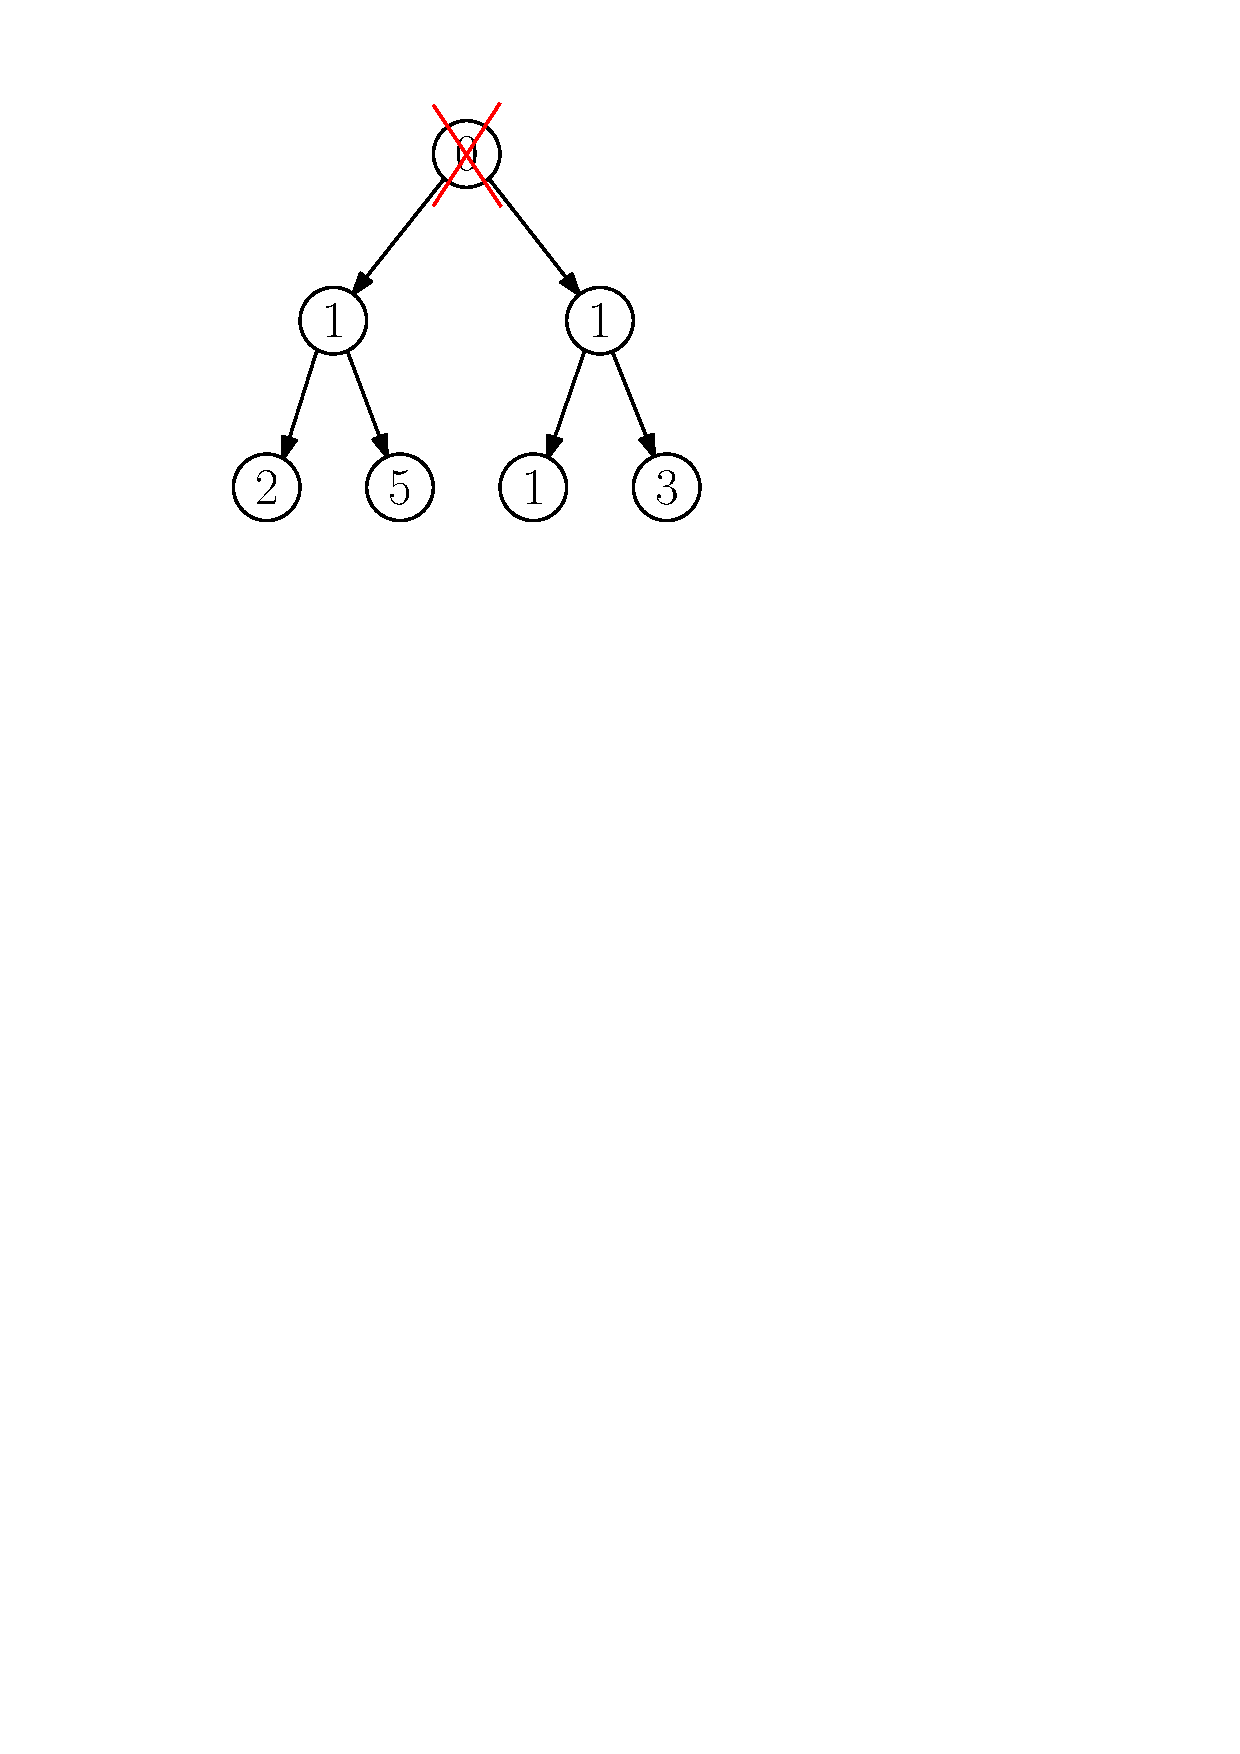
\includegraphics[scale=.5]{ch01_odebirani_1}
    \end{subfigure}
    \begin{subfigure}{5cm}
        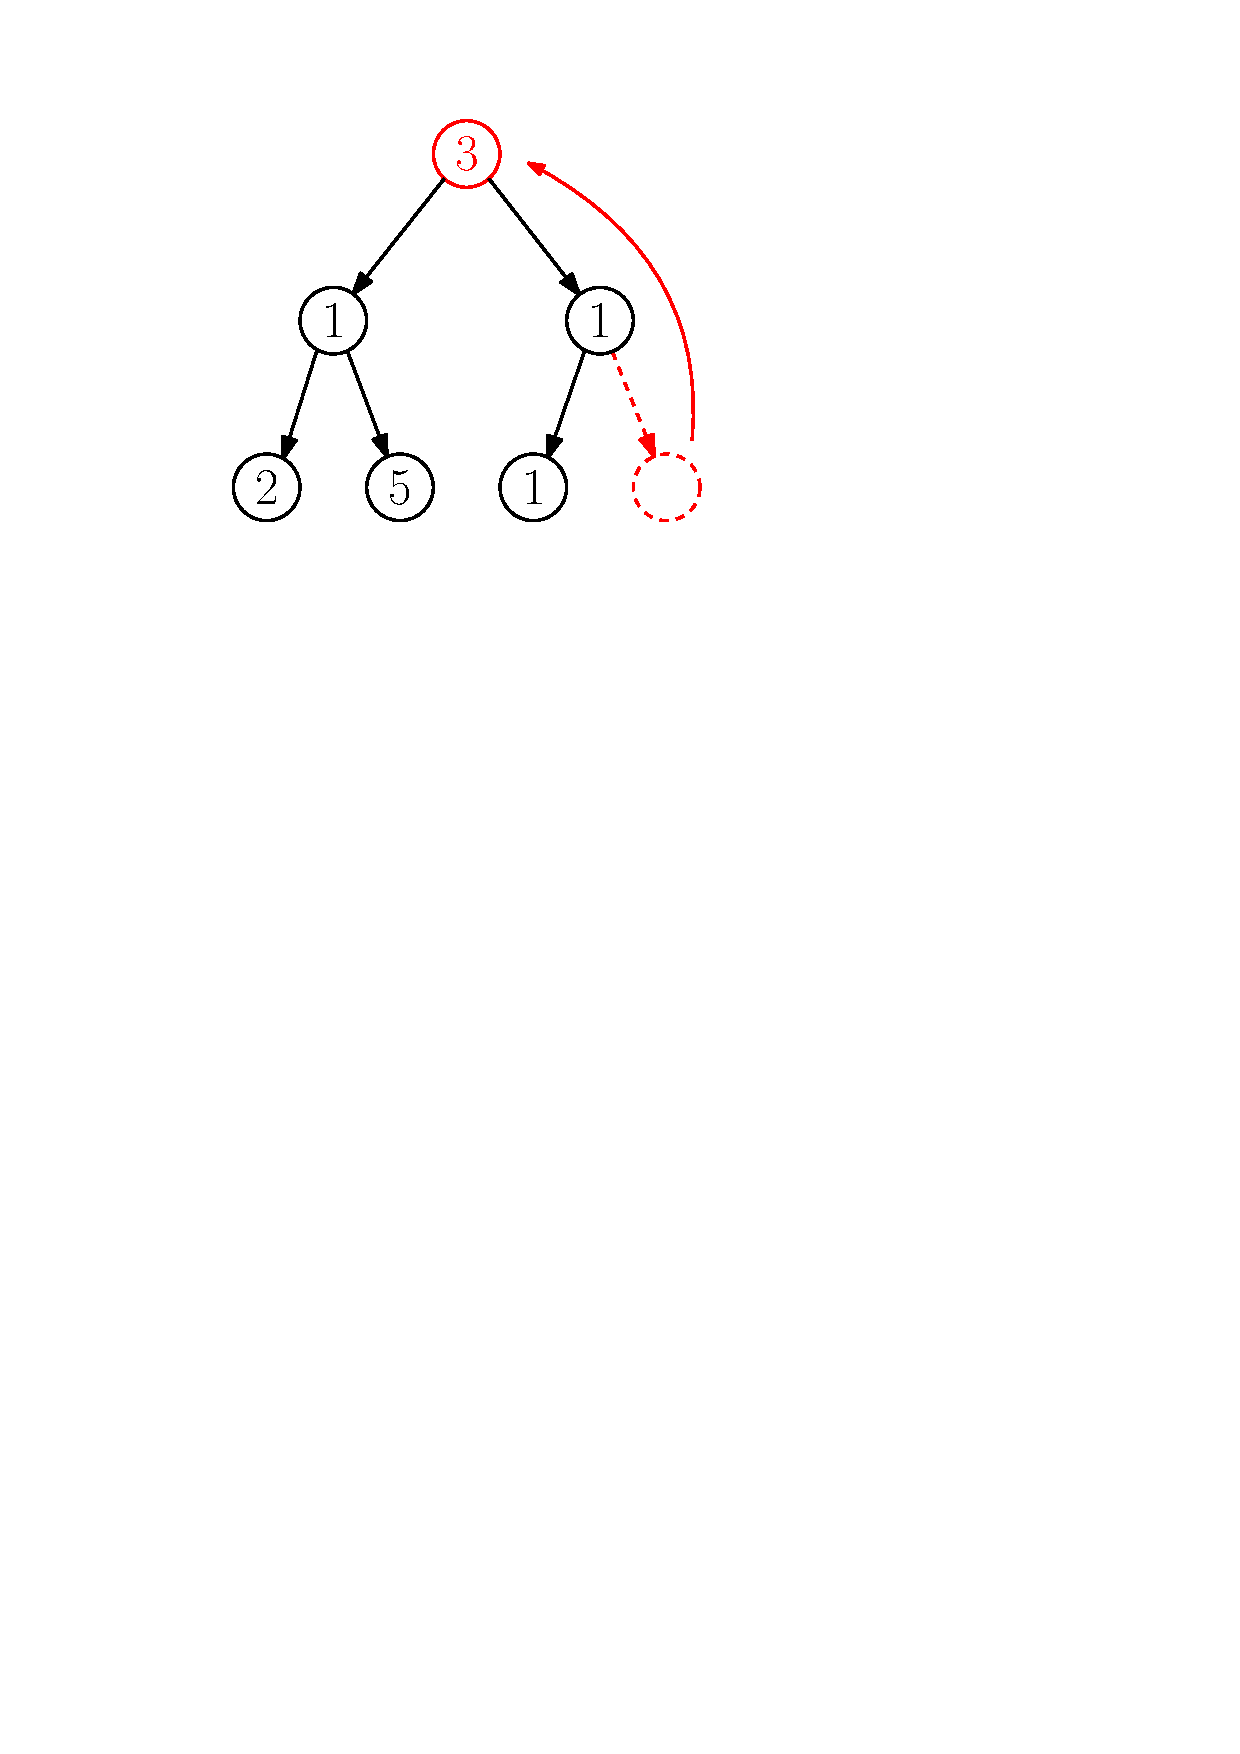
\includegraphics[scale=.5]{ch01_odebirani_2}
    \end{subfigure}
    \begin{subfigure}{5cm}
        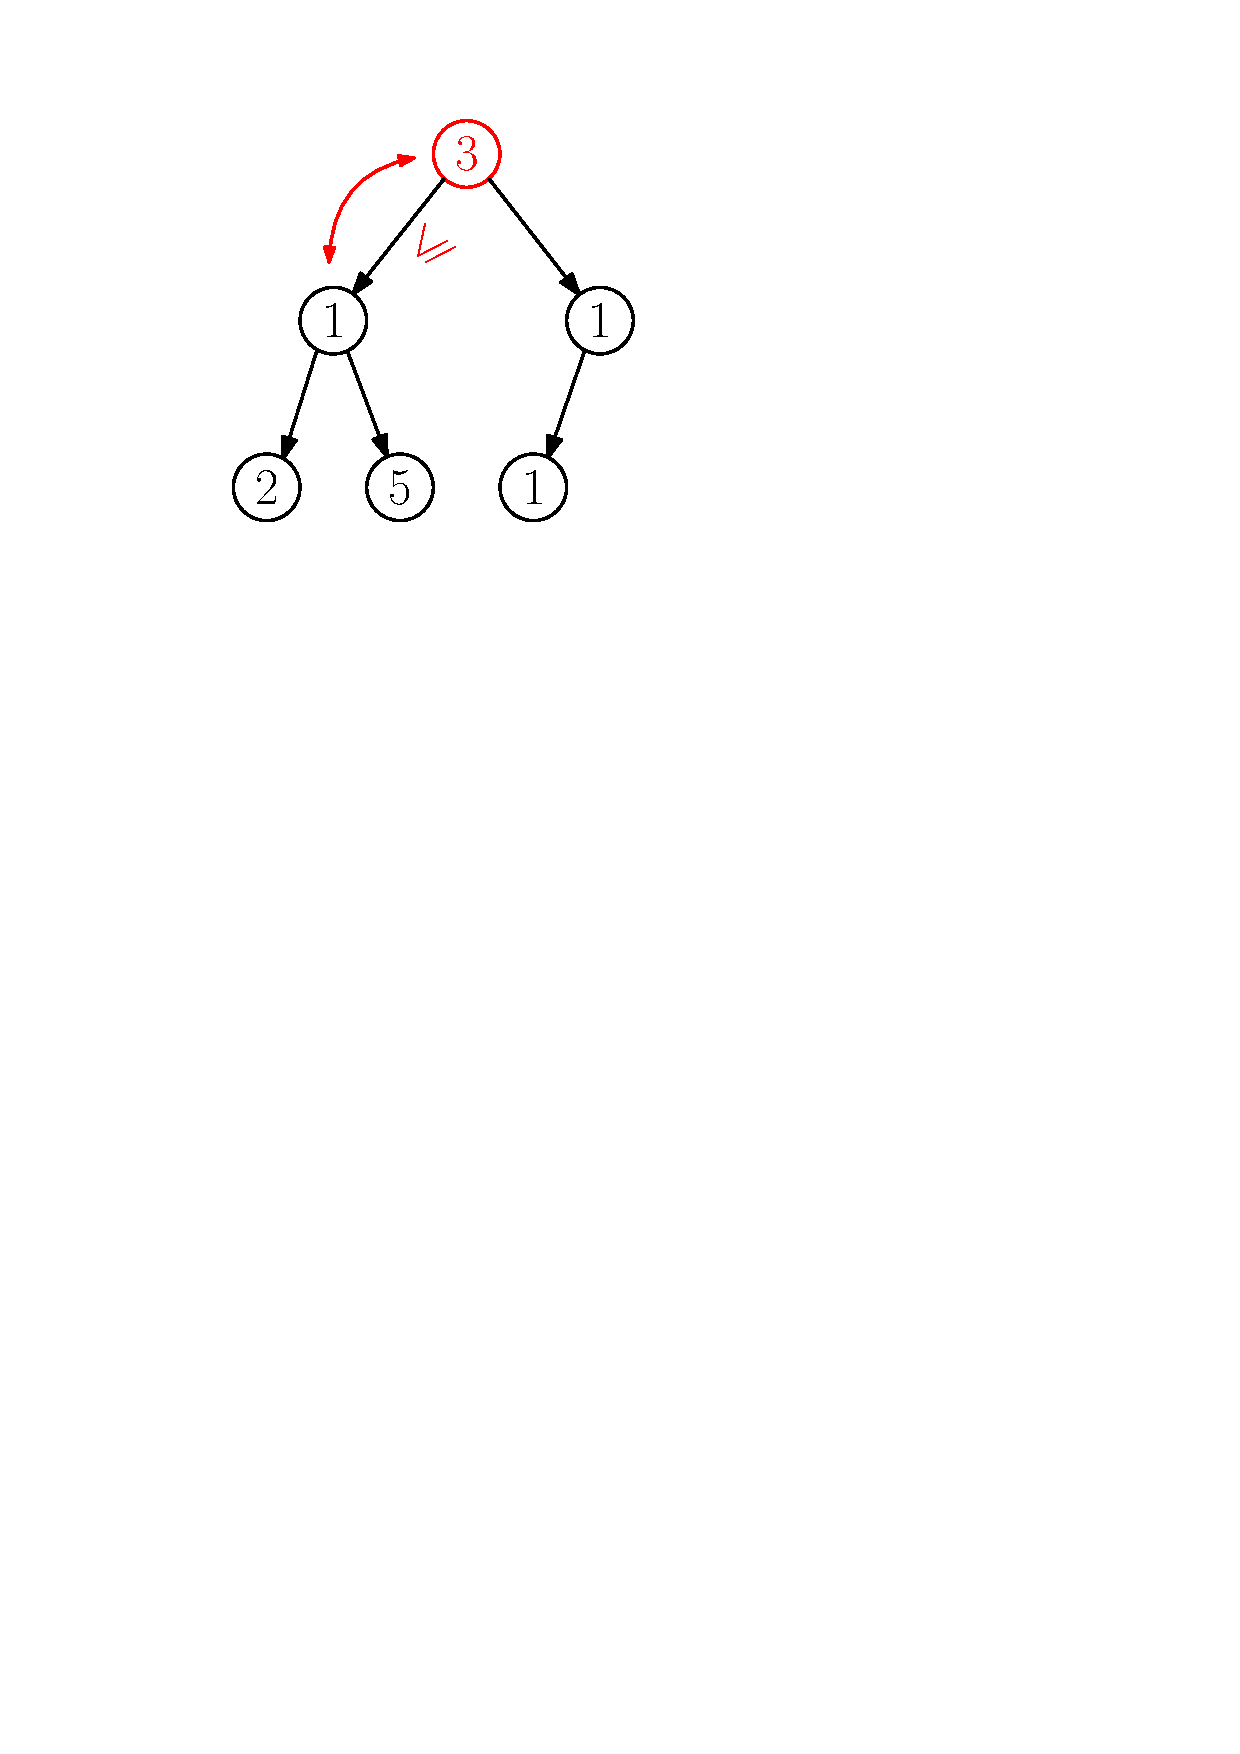
\includegraphics[scale=.5]{ch01_odebirani_3}
    \end{subfigure}
    \begin{subfigure}{5cm}
        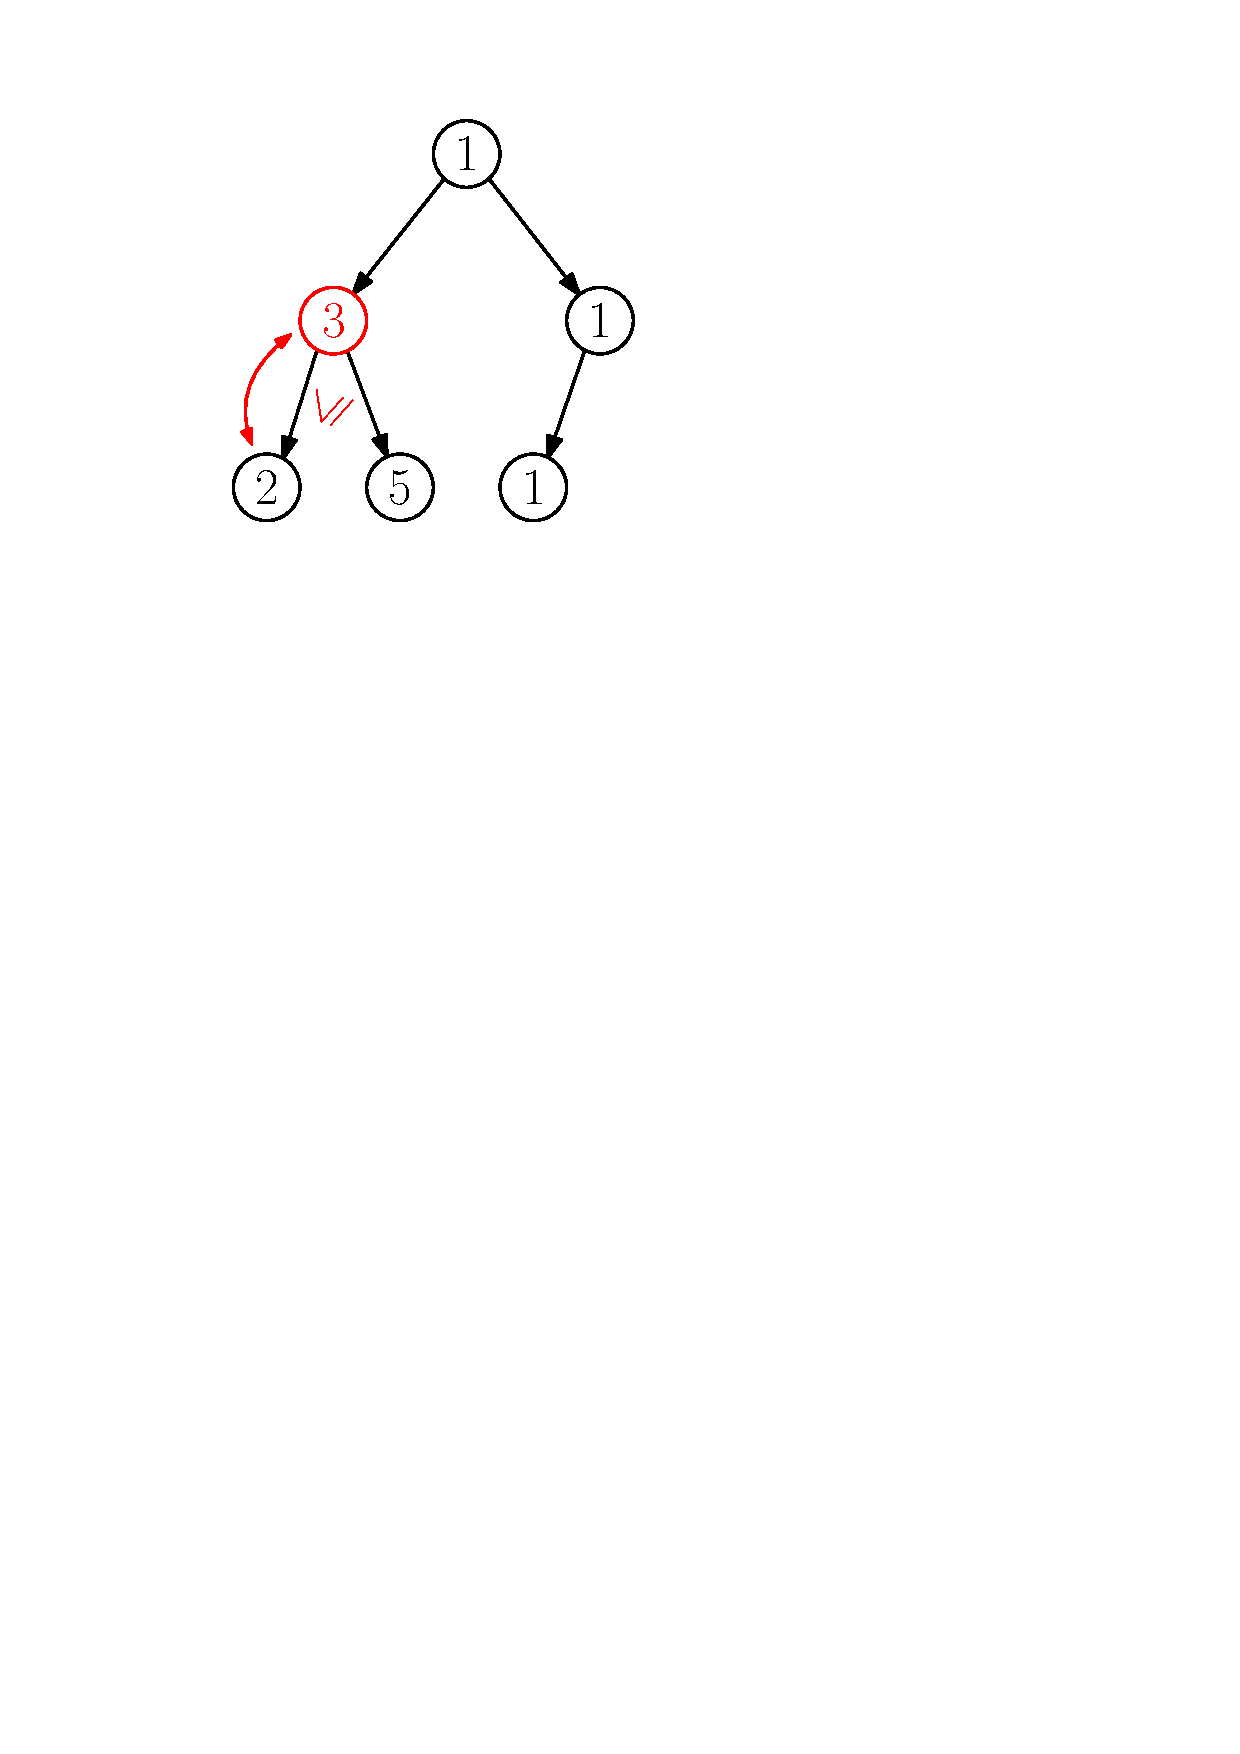
\includegraphics[scale=.5]{ch01_odebirani_4}
    \end{subfigure}
    \begin{subfigure}{5cm}
        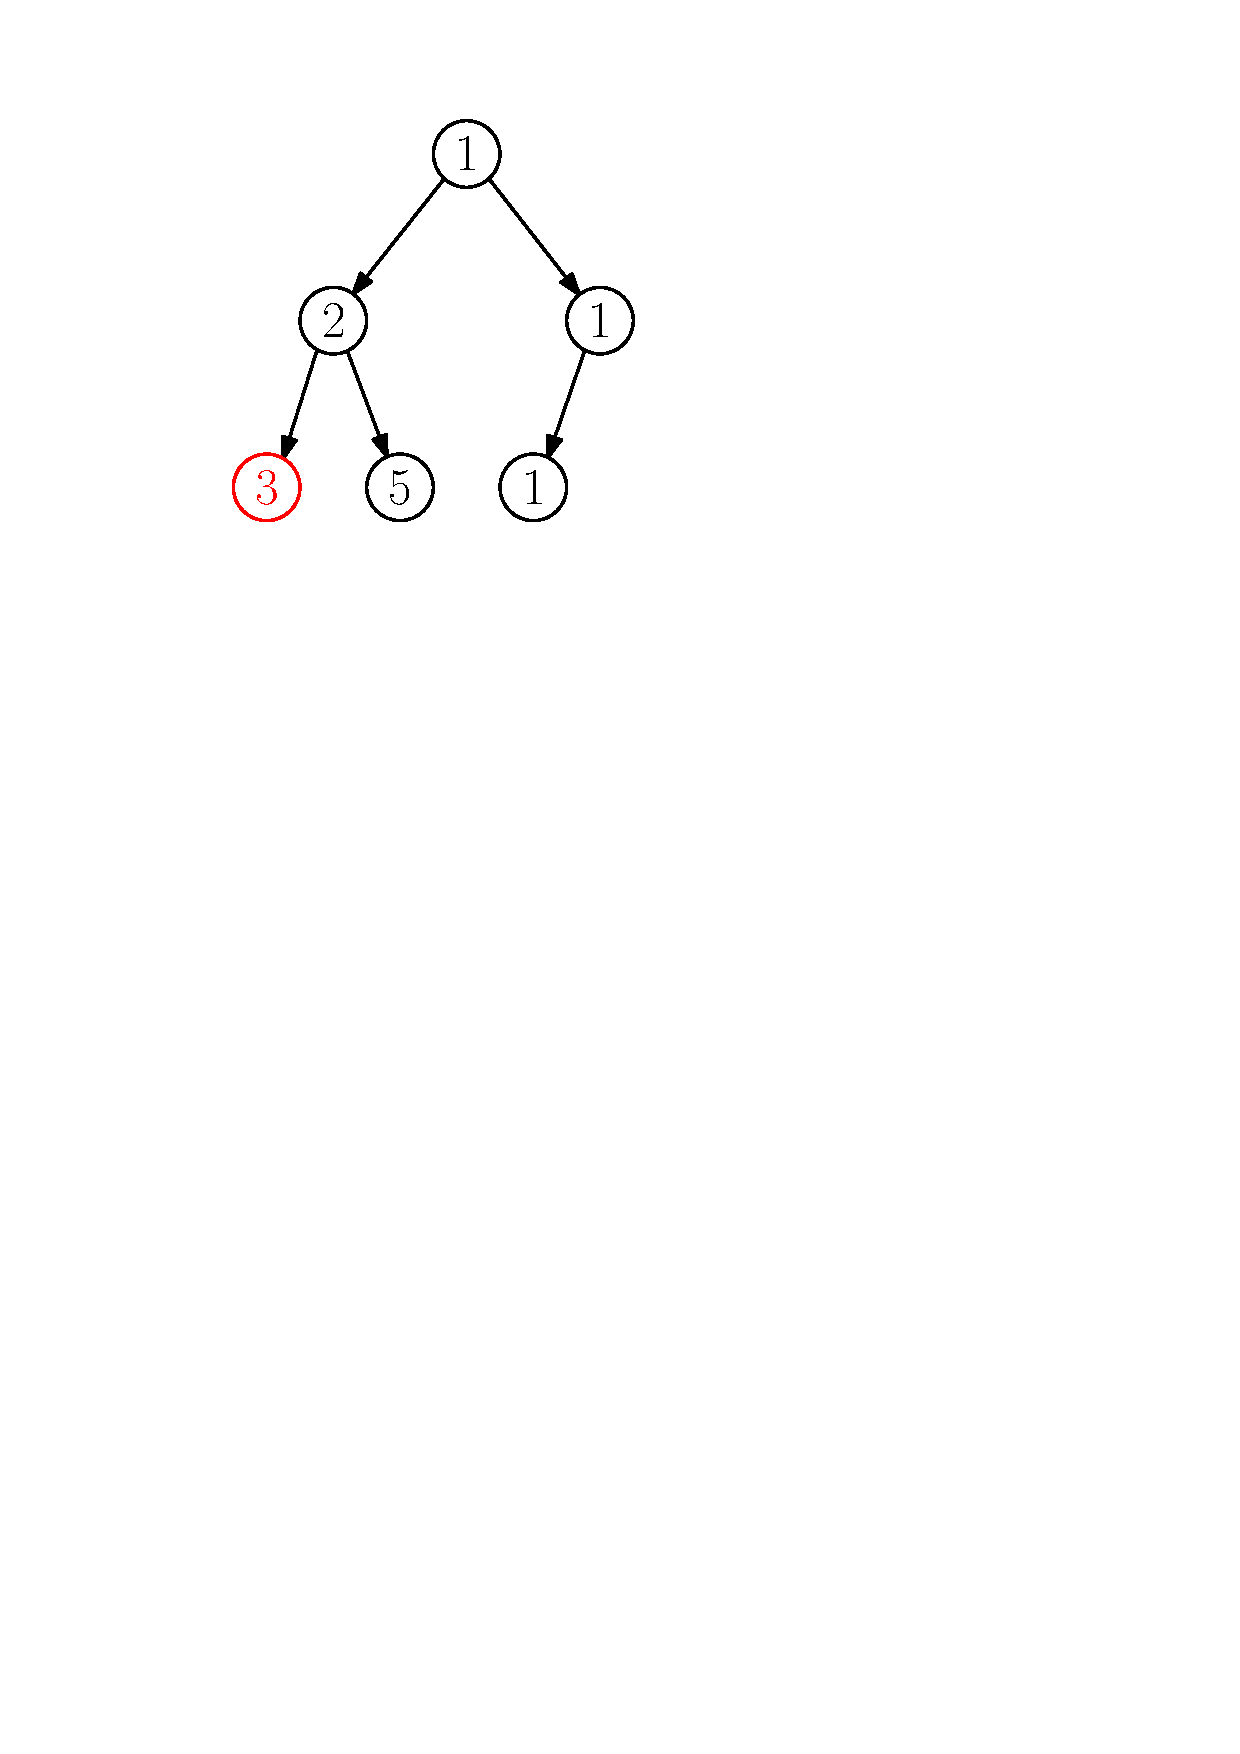
\includegraphics[scale=.5]{ch01_odebirani_5}
    \end{subfigure}
    \caption{Odebírání vrcholu (kořene) s minimálním klíčem.}
    \label{fig:odebirani_vrcholu_halda}
\end{figure}
V bodech můžeme zapsat celou operaci následovně:
\begin{itemize}
    \item Smažeme kořen a nahradíme jej nejlevějším vrcholem na poslední hladině.
    \item Tento vrchol (resp. jeho klíč) porovnáme s jeho syny a případně prohodíme s tím, jehož klíč je menší.
    \item Opakujeme druhý krok.
\end{itemize}
Operacím, které jsme prezentovali při vkládání vrcholu, resp. odebírání minima z haldy, kdy vrchol "probublával" nahoru, resp. dolů, se někdy nazývají \textsc{BubbleUp} a \textsc{BubbleDown}. Ještě se nám budou hodit u operací \textsc{Increase} a \textsc{Decrease}.

\subsubsection{Zvýšení a snížení hodnoty klíče ve vrcholu}

Poslední dvojice operací, která se nám bude hodit, je zvýšení (\textsc{Increase}) a snížení (\textsc{Decrease}) hodnoty klíče ve vybraném vrcholu. K tomu potřebujeme akorát vyřešit, jak budeme k vrcholům přistupovat. Podle klíče vyhledávat neumíme, ale můžeme si zavést např. pomocný slovník, který budeme "adresovat" pomocí příslušného vrcholu a vracenou hodnotou bude klíč ve vrcholu. Takto spotřebujeme navíc pouze $\bigO{n}$ paměti, kde $n$ je počet vrcholů v haldě.

Realizace samotných operací je již jednoduchá. Pokud protovedeme \textsc{Increase} klíče v určitém vrcholu, pak z důvodu, že klíče v synech vrcholu jsou stejné nebo větší, se halda může pokazit pouze "směrem dolů". Tedy provedeme nám již známé prohazování vrcholu s jeho syny, dokud nebude halda opravena (\textsc{BubbleDown}), stejně jako v případě odebírání kořene (\textsc{ExtractMin}).

Operaci \textsc{Decrease} provedeme zcela stejně, akorát nyní se halda bude kazit "směrem nahoru", takže provedeme \textsc{BubbleUp}, jako při vkládání nového vrcholu (\textsc{Insert}).
\notebox{V případě \emph{maximové binární haldy} by operace vypadaly zcela stejně, akorát při operaci \textsc{Increase} budeme opravovat haldu směrem nahoru a u \textsc{Decrease} směrem dolů.}

\subsubsection{Časové složitosti operací}

Pojďme si nyní rozebrat časové složitosti zmíněných operací \textsc{Insert}, \textsc{Min}, \textsc{ExtractMin}, \textsc{Increase} a \textsc{Decrease} a podívat se, jak moc jsme si pomohli oproti práci s polem (seznamem). Pokud se pozorně podíváme na operace popsané výše, je zjevné, že nejvíce bude naše operace zpomalovat ono "probublávání" vrcholu při opravování haldy (vyjma operace \textsc{Min}, kde jen přečteme klíč v kořeni), tj. \textsc{BubbleUp} a \textsc{BubbleDown}. Na nich bude celková časová složitost záviset.
\tipbox{Všimněme si, že po každém prohození vrcholů při \textsc{BubbleUp} nebo \textsc{BubbleDown} se vrchol posune o jednu hladinu výše/níže.}
Víme tak, že při opravování haldy se vrchol může posunout \emph{maximálně o počet hladin}, který má daná halda. Časová složitost daných operací bude tak závislá na jejich počtu. Tím jsme se dostali o trochu blíže řešení, ale rádi bychom věděli, jak se bude době trvání daných operací měnit v závislosti na \emph{počtu vrcholů v haldě}, nikoliv počtu hladin. Mezi těmito proměnnými však existuje hezká závislost.

Dejme tomu, že naše halda má $n$ vrcholů v celkově $h$ hladinách, přičemž poslední hladina \emph{je plně obsazena} (viz obrázek \ref{fig:halda_hladiny}). (Mohlo by se, v obecném případě, samozřejmě stát, že poslední hladina plně obsazena nebude, ale jediné, co se tím změní, bude, že mezi $n$ a výsledným výrazem bude místo rovnosti nerovnost. S plnou hladinou se nám ale bude lépe počítat, protože při analýze časové složitost nás zajímá nejhorší možný případ.) Pokud budeme mít haldu s jednou hladinou, bude mít pouze jeden vrchol, a to kořen. S dvěma hladinami budou již 3 vrcholy v haldě. S třemi hladinami jich bude 7, atd (viz tabulka \ref{tab:halda_vrcholy_hladiny}).
\begin{table}[h]
    \centering
    \begin{tabular}{|l|c|c|c|c|c|c|}
        \hline
        Počet hladin $h$  & 1 & 2 & 3 & 4  & 5  & 6  \\ \hline
        Počet vrcholů $n$ & 1 & 3 & 7 & 15 & 31 & 63 \\ \hline
    \end{tabular}
    \caption{Vztah mezi počtem hladin $h$ a počtem vrcholů $n$ v plně obsazené haldě.}
    \label{tab:halda_vrcholy_hladiny}
\end{table}
\begin{figure}[h]
    \centering
    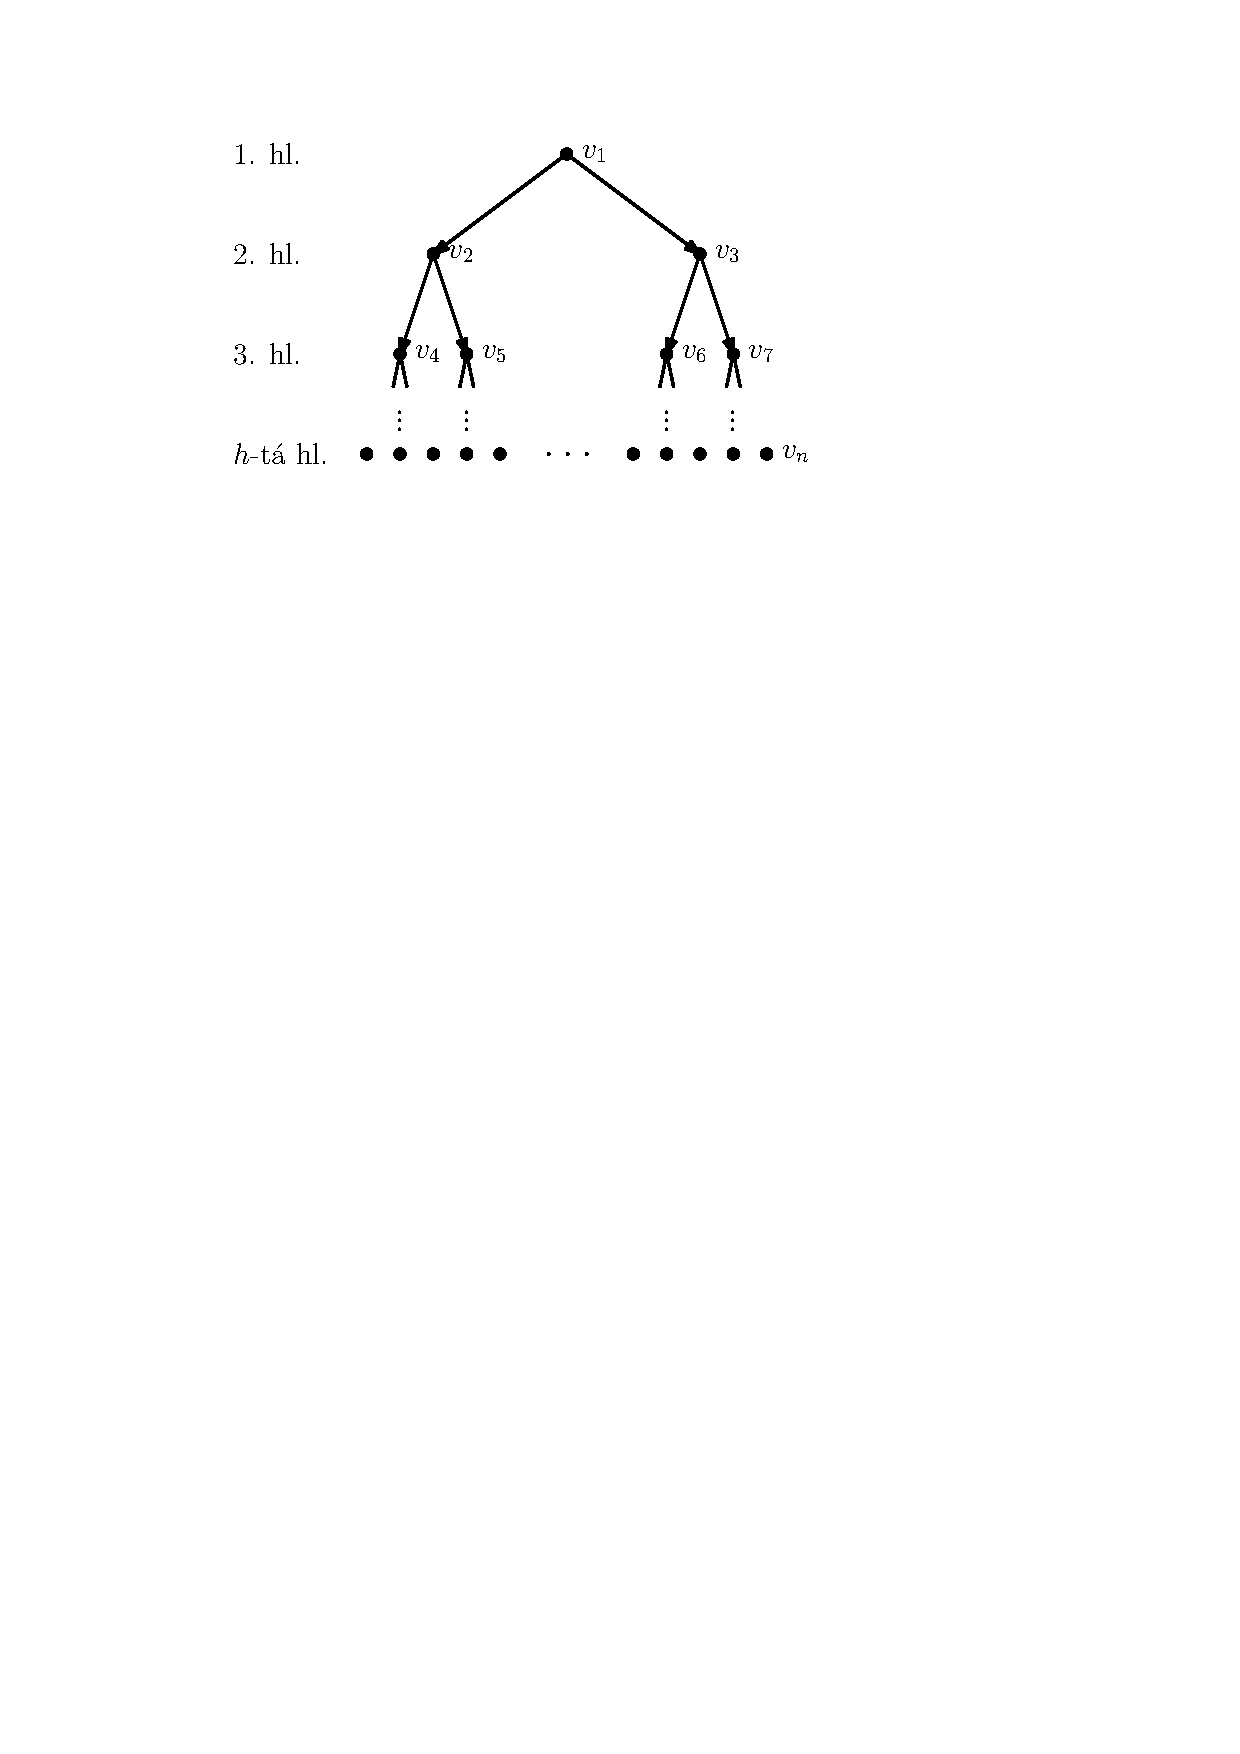
\includegraphics[scale=0.75]{ch01_halda_hladiny}
    \caption{Odebírání vrcholu (kořene) s minimálním klíčem.}
    \label{fig:halda_hladiny}
\end{figure}
Z tabulky \ref{tab:halda_vrcholy_hladiny} si můžeme všimnout, že počet vrcholů je vždy \emph{mocnina dvojky snížená o jedna}. Výsledná závislost je tedy $n=2^h-1$. V případě, že by poslední hladina nebyla plně obsazena, by se rovnost změnila v nerovnost, tj. $n\leqslant2^h-1$. Tím máme již vše připravené k tomu, abychom odvodili časovou složitost daných operací.
\begin{theorem}[Složitost operací v binární haldě]
    Operace \textsc{Insert}, \textsc{ExtractMin}, \textsc{Increase} a \textsc{Decrease} mají časovou složitost $\bigO{\log{n}}$. Operace \textsc{Min} má časovou složitost $\bigO{1}$.
\end{theorem}
\begin{proof}
    V případě \textsc{Min} je to jednoduché, zkrátka jen přečteme klíč v kořeni, což zjevně potrvá $\bigO{1}$. U zbývajících operací opravujeme haldu pomocí \textsc{BubbleUp} a \textsc{BubbleDown}. Předpokládejme, nastal nejhorší možný případ, tj. halda má $h$ hladin a je plně obsazena (tzn. včetně poslední hladiny). Víme, že "probublání" vrcholu haldou nahoru/dolů potrvá řádově $\bigO{h}$. My však víme, že $n=2^h-1$. Tedy zde bude stačit, když si vyjádříme $h$ z rovnosti.
    \[n=2^h-1 \iff 2^h=n+1 \iff h=\log_2{(n+1)}\stackrel{\texttt{*}}{=}\dfrac{1}{\log{2}}\cdot\log{(n+1)}.\]
    (V rovnosti \texttt{*} jsme využili vzorec $\log_b{a}=\log{a}/\log{b}$.) Operace \textsc{BubbleUp} a \textsc{BubbleDown} tedy potrvají
    \[\bigO{h}=\bigO{\dfrac{1}{\log{2}}\cdot\log{(n+1)}}\stackrel{\texttt{*}}{=}\bigO{\log{n}}.\]
    (V \texttt{*} je jednička v logaritmu zanedbatelná v rámci $\mathcal{O}$-notace. Výraz $1/\log{2}$ představuje konstantu a tudíž je též zanedbatelný.) Tedy operace \textsc{Insert}, \textsc{ExtractMin}, \textsc{Increase} a \textsc{Decrease} mají logaritmickou časovou složitost.
\end{proof}
Zkusme si na závěr udělat menší porovnání oproti poli, se kterým jsme začínali (viz tabulka \ref{tab:halda_pole_operace}).
\begin{table}[h]
    \centering
    \begin{tabular}{l|ccccc}
                  & \textsc{Insert} & \textsc{Min} & \textsc{ExtractMin} & \textsc{Increase} & \textsc{Decrease} \\\hline
    Pole (seznam) & $\bigO{1}$                       & $\bigO{n}$                    & $\bigO{n}$                           & $\bigO{1}$                         & $\bigO{1}$                         \\
    Binární halda & $\bigO{\log{n}}$                 & $\bigO{1}$                    & $\bigO{\log{n}}$                     & $\bigO{\log{n}}$                   & $\bigO{\log{n}}$                  
    \end{tabular}
    \caption{Porovnání časových složitostí operací v haldě a v poli.}
    \label{tab:halda_pole_operace}
\end{table}
Logaritmická časová složitost je určitě lepší, než lineární, je však vidět, že jsme si zároveň pohoršili v případě vkládání a úpravy hodnot klíčů. Je tomu tak z důvodu, že pole má svou výhodu v téměř nulové režii, kdežto halda (kvůli své pevně definované struktuře) spotřebuje nějaký čas, aby byla uvedena do korektního stavu.
